\section{Einf\"uhrung in Finite Differenzen Methoden}
Den Finiten Differenzen Methoden liegt eine punktuelle Taylor-Entwicklung zugrunde. Die Approximationsordnung des resultierenden Differenzenquotients ist dabei ein Ma\ss{}stab f\"ur die Genauigkeit des Verfahrens.

\begin{equation}
	u(x+\dex) = u(x) + \dex\frac{\partial u}{\pet}\bigg|_{x} + \frac{\dex^2}{2}\frac{\partial^2 u}{\pex^2}\bigg|_x + \dots
\end{equation}
\begin{equation}
	\Rightarrow ~~~ \frac{\partial u}{\pex}\bigg|_x = \frac{u(x + \dex ) - u(x)}{\dex} - \frac{\dex}{2}\frac{\partial^2 u}{\pex^2}\bigg|_x + \dots
\end{equation}

\vspace{-1.6em}
\begin{tikzpicture}
	\centering
	\node[anchor=south west,inner sep=0] (Bild) at (0,0){};
	\begin{scope}[x=(Bild.south east),y=(Bild.north west)]
		\draw [ultra thick] [->] (280,0) -- (230,10) node [pos=0,below] {Restterme};
	\end{scope}
\end{tikzpicture}

\begin{equation}
	\Rightarrow ~~~ \frac{\partial u}{\pex}\bigg|_x = \frac{u(x + \dex ) - u(x)}{\dex} + O(\dex) \approx \frac{u(x + \dex ) - u(x)}{\dex} ~~~~ (\textrm{mit } O(\dex ) \textrm{ als Landau Symbol})
\end{equation}

\vspace{-2.5em}
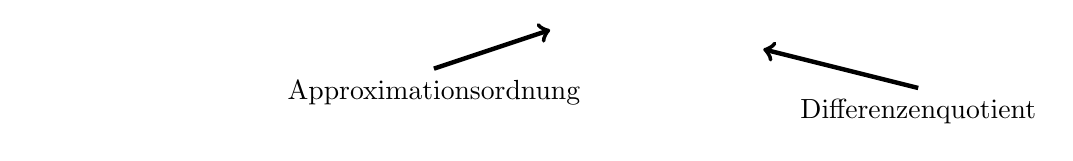
\begin{tikzpicture}
	\centering
	\node[anchor=south west,inner sep=0] (Bild) at (0,0){};
	\begin{scope}[x=(Bild.south east),y=(Bild.north west)]
		\draw [ultra thick] [->] (105,5) -- (135,15) node [pos=0,below] {Approximationsordnung};
		\draw [ultra thick] [->] (230,0) -- (190,10) node [pos=0,below] {Differenzenquotient};
	\end{scope}
\end{tikzpicture}

Die Finiten Differenzen lassen sich nach mehreren Gesichtspunkten unterscheiden: 
\begin{itemize}
	\item Ordnung 
	\item Gitterform (\"Aquidistant oder nicht)
	\item Rechenrichtung:
	\begin{itemize}
		\item R\"uckw\"arts (implizit)
		\item Vorw\"arts (explizit)
		\item Zentral (Symmetrisch)
	\end{itemize}
\end{itemize}

Die Finiten Differenzen, und damit auch die Taylerentwicklung l\"asst sich in h\"ohere Ordnungen entwickeln. F\"ur die Ordnung $n$ werden $n+1$ St\"utzpunkte auf dem Gitter ben\"otigt.
\par
Dabei existieren in der ersten Ordnung nur Vorw\"arts- und R\"uckw\"artsdifferenzen, zentrale Differenzen existieren erst ab der Zweiten Ordnung.
\par
Im folgenden werden einige Beispiele Aufgezeigt, welche diese Unterscheidungen zeigen:


\newpage

\textbf{Finite Differenzen erster Ordnung:}
\begin{multicols}{2}
\vspace{-2em}
\includegraphics[width=0.5\textwidth]{firstdiffmet}


\vfill\null
\columnbreak

\textbf{vorw\"arts:}
\vspace{-1.5em}
\begin{multline*} 
	u_{i+1}(x_i+\dex) = u_i(x) + \dex\frac{\partial u}{\pex}\bigg|_{x_i} + O(\dex^2) \\ 
	\Rightarrow \frac{\partial u}{\pex}\bigg|_{x_i} = \frac{u_{i+1} - u_i}{\dex} + O(\dex)
\end{multline*}
\vspace{-1.5em}
\textbf{r\"uckw\"arts:}
\begin{multline*} 
	u_{i-1}(x_i-\dex) = u_i(x) - \dex\frac{\partial u}{\pex}\bigg|_{x_i} + O(\dex^2) \\ \Rightarrow \frac{\partial u}{\pex}\bigg|_{x_i} = \frac{u_{i} - u_{i-1}}{\dex} + O(\dex)
\end{multline*}

\end{multicols}


\textbf{Finite Differenzen zweiter Ordnung mit \"aquidistantem Gitter:}
\begin{multicols}{2}
\vspace{-2em}
\includegraphics[width=0.5\textwidth]{seconddiffmet}

\vfill\null
\columnbreak

\textbf{zentral:}
\vspace{-1.5em}
\begin{align*} 
	u_{i+1} &= u_i + \dex\frac{\partial u}{\pex}\bigg|_{x_i} + \frac{\dex}{2}\frac{\partial^2 u}{\pex^2}\bigg|_{x_i} + O(\dex^3) \\
	u_{i+1} &= u_i + \dex\frac{\partial u}{\pex}\bigg|_{x_i} + O(\dex^3) \\
	\Rightarrow \frac{\partial u}{\pex}\bigg|_{x_i} &= \frac{\dex^2_{i-1} u_{i+1} + u_i (\dex^2_i - \dex^2_{i-1}) - \dex^2_i u_{i-1}}{\dex} \\ &+ O(\dex^2)
\end{align*}
\vspace{-1em}
\textbf{r\"uckw\"arts (vorw\"arts analog):}
\begin{align*} 
	u_{i-1} &= u_i - \dex\frac{\partial u}{\pex}\bigg|_{x_i} + \frac{\dex^2}{2}\frac{\partial^2u}{\dex^2} + O(\dex^3) \\
	u_{i-2} &= u_i - 2\dex\frac{\partial u}{\pex}\bigg|_{x_i} + \frac{4\dex^2}{2}\frac{\partial^2 u}{\dex^2}\bigg|_{x} + O{\dex^3}\\
	\Rightarrow \frac{\partial u}{\pex}\bigg|_{x_i} &= \frac{3u_{i} - 4u_{i-1} + u_{i-2}}{2\dex} + O(\dex^2)
\end{align*}

\end{multicols}



\textbf{Finite Differenzen zweiter Ordnung mit nicht-\"aquidistantem Gitter:}
\begin{multicols}{2}
\vspace{-2em}
\includegraphics[width=0.5\textwidth]{seconddiffmet_no_equal}

\vfill\null
\columnbreak

\textbf{zentral:}
\vspace{-1.5em}
\begin{align*} 
	u_{i+1} &= u_i + \dex\frac{\partial u}{\pex}\bigg|_{x_i} + \frac{\dex^2}{2}\frac{\partial^2 u}{\pex^2}\bigg|_{x_i} + O(\dex^3) \\
	u_{i-1} &= u_i - \dex_{i-1}\frac{\partial u}{\pex}\bigg|_{x_i} + \frac{\dex^2_{i-1}}{2}\frac{\partial^2 u}{\pex^2}\bigg|_{x_i} + O(\dex^3)\\
	\Rightarrow \frac{\partial u}{\pex}\bigg|_{x_i} &= \frac{\dex^2_{i-1}u{i+1} + u_i(\dex^2_i - \dex^2_{i-1}) - \dex^2_i u_{i-1}}{\dex_i \dex_{i-1} (\dex_i + \dex_{i-1})}\\
	&+ O(\dex^2)
\end{align*}

\end{multicols}

\newpage

\subsection{Zeitschritt (stepping) Ansatz}
Im folgenden wird als Rechenbeispiel die Skalare Wellengleichung~\ref{eq:scalarwave} verwendet.
\begin{equation}
	\frac{\partial u}{\pet} + a\frac{\partial u}{\pex} = 0~~~~~\textrm{mit}~~~~~
	u(x,0) = u_0(x)
	\label{eq:scalarwave} 
\end{equation}

Die Allgemeine L\"osung dazu ist in~\ref{eq:gensolu} gegeben.
\begin{equation}
	u(x,t) = u_0(x - at)~~~~~\textrm{bzw.}~~~~~
	u(x,t + \delt) = u_0(x - a\delt,t)
	\label{eq:gensolu} 
\end{equation}

\begin{multicols}{2}
	\textbf{Explizit}
	\begin{itemize}
		\item Nutze FD zur Zeitableitung um Unbekannte $u^{n+1}$ zu finden
		\item Nutze FD zur Ortsableitung am alten Zeitschritt $t^n$
	\end{itemize}
	Es ergibt sich die Formel:\\
	\includegraphics[width=0.5\textwidth]{stepping_expl}
	Die neue L\"osung bei $n+1$ h\"angt also nur von alten L\"osungen auf vorherigen Zeitschritten ab.

% \vfill\null
\columnbreak

	\textbf{Implizit}
	\begin{itemize}
		\item Nutze FD zur Zeitableitung um Unbekannte $u^{n+1}$ zu finden
		\item Nutze FD zur Ortsableitung am alten Zeitschritt $t^{n+1}$
	\end{itemize}
	Es ergibt sich die Formel:\\
	\includegraphics[width=0.5\textwidth]{stepping_impl}
	Die neue L\"osung bei $n+1$ h\"angt also von alten L\"osungen auf vorherigen Zeitschritten und von der neuen, aktuellen L\"osung ab.
\end{multicols}

\subsection{Verschiedene Schrittverfahren}
\textbf{Euler-Explizit-Vorw\"arts}
\begin{multicols}{2}
	\includegraphics[width=0.25\textwidth]{euler_ef}
\columnbreak
	\begin{multline*}
		\frac{u^{n+1}_i - u^n_i}{\delt} + a\frac{u^{n}_{i+1} - u^n_i}{\dex} + O(\delt) + O(\dex) = 0 \\
		\Rightarrow u^{n+1}_i = u^n_i - \frac{a\delt}{\dex}(u^n_{i+1} - u^n_i)
	\end{multline*}
	Zeitschritte = 2\\
	Erste Ordnung in $\delt$ und $\dex$: 
	\begin{itemize}
		\item konditionell stabil f\"ur $a<0$
		\item instabil f\"ur $a>0$
	\end{itemize}
\end{multicols}

\newpage

\textbf{Euler-Explizit-R\"uckw\"arts}
\begin{multicols}{2}
	\includegraphics[width=0.25\textwidth]{euler_eb}
\columnbreak
	\begin{multline*}
		\frac{u^{n+1}_i - u^n_i}{\delt} + a\frac{u^{n}_i - u^n_{i-1}}{\dex} + O(\delt) + O(\dex) = 0 \\
		\Rightarrow u^{n+1}_i = u^n_i - \frac{a\delt}{\dex}(u^n_{i} - u^n_{i-1})
	\end{multline*}
	Zeitschritte = 2\\
	Erste Ordnung in $\delt$ und $\dex$: 
	\begin{itemize}
		\item konditionell stabil f\"ur $a>0$
		\item instabil f\"ur $a<0$
	\end{itemize}
\end{multicols}

\textbf{Euler-Implizit-R\"uckw\"arts}
\begin{multicols}{2}
	\includegraphics[width=0.25\textwidth]{euler_ib}
\columnbreak
	\begin{multline*}
		\frac{u^{n+1}_i - u^n_i}{\delt} + a\frac{u^{n+1}_i - u^{n+1}_{i-1}}{\dex} + O(\delt) + O(\dex) = 0 \\
		\Rightarrow u^{n+1}_i = u^n_i - \frac{a\delt}{\dex}(u^{n+1}_{i} - u^{n+1}_{i-1})
	\end{multline*}
	Zeitschritte = 2\\
	Erste Ordnung in $\delt$ und $\dex$: 
	\begin{itemize}
		\item stabil f\"ur $a>0$
		\item instabil f\"ur $a<0$
	\end{itemize}
\end{multicols}

\textbf{Euler-Explizit-Zentral}
\begin{multicols}{2}
	\includegraphics[width=0.25\textwidth]{euler_ec}
\columnbreak
	\begin{multline*}
		\frac{u^{n+1}_i - u^n_i}{\delt} + a\frac{u^{n}_{i+1} - u^{n}_{i-1}}{2\dex} + O(\delt) + O(\dex^2) = 0 \\
		\Rightarrow u^{n+1}_i = u^n_i - \frac{a\delt}{2\dex}(u^{n}_{i+1} - u^{n}_{i-1})
	\end{multline*}
	Zeitschritte = 2\\
	Erste Ordnung in $\delt$, zweite Ordnung in $\dex$: 
	\begin{itemize}
		\item immer instabil
	\end{itemize}
\end{multicols}

\textbf{Zentral-Explizit-R\"uckw\"arts}
\begin{multicols}{2}
	\includegraphics[width=0.25\textwidth]{central_eb}
\columnbreak
	\begin{multline*}
		\frac{u^{n+1}_i - u^{n-1}_i}{2\delt} + a\frac{u^{n}_{i} - u^{n}_{i-1}}{\dex} + O(\delt^2) + O(\dex) = 0 \\
		\Rightarrow u^{n+1}_i = u^{n-1}_i - \frac{2a\delt}{\dex}(u^{n}_{i} - u^{n}_{i-1})
	\end{multline*}
	Zeitschritte = 3\\
	Erste Ordnung in $\dex$, zweite Ordnung in $\delt$: 
	\begin{itemize}
		\item immer instabil
	\end{itemize}
\end{multicols}

\textbf{Zentral-Explizit-R\"uckw\"arts}
\begin{multicols}{2}
	\includegraphics[width=0.25\textwidth]{central_eb}
\columnbreak
	\begin{multline*}
		\frac{u^{n+1}_i - u^{n-1}_i}{2\delt} + a\frac{u^{n}_{i+1} - u^{n}_{i-1}}{\dex^2} + O(\delt^2) + O(\dex) = 0 \\
		\Rightarrow u^{n+1}_i = u^{n-1}_i - \frac{2a\delt}{\dex}(u^{n}_{i+1} - u^{n}_{i-1})
	\end{multline*}
	Zeitschritte = 3\\
	Zweite Ordnung in $\delt$ und $\dex$: 	
	\begin{itemize}
		\item konditionell stabil
	\end{itemize}
\end{multicols}

\begin{itemize}
	\item Explizite vorw\"arts Verfahren funktionieren nur f\"ur $a<0$
	\item Explizite r\"uckw\"arts Verfahren funktionieren nur f\"ur $a>0$
	\item Explizite Verfahren k\"onnen nur konditionell stabil werden
	\item Implizite Verfahren k\"onnen auch immer instabil sein
\end{itemize}

\subsection{Fehleranalyse}
Es gibt zwei haupts\"achliche Fehlerquellen in Simulationen:
\begin{multicols}{2}
Numerische Rundungsfehler:
\begin{itemize}
	\item N\"aherungsweise Darstellung von Zahlen und Operationen in Computern
	\item H\"angt von der Genauigkeit der Rechenmaschine und der Anzahl an Operationen ab.
\end{itemize}
\columnbreak
Diskretisierungsfehler:
\begin{itemize}
	\item N\"aherung von Ableitungen durch Differenzenquotienten
	\item Abh\"angig von Gittergr\"o\ss{}e und Zeitschritten ($\dex$, $\delt$)
	\item Abh\"angig von der verwendeten FD Methode und deren Kombination.
\end{itemize}
\end{multicols}

\subsubsection{Globaler Fehler}
Der Globale Fehler beschreibt die Abweichung der exakten und der numerischen L\"osung in jedem Zeitschritt auf jedem Gitterpunkt.
\begin{itemize}
	\item Nicht anwendbar wenn die exakte L\"osung unbekannt ist
	\item Punktweise Definition: Skalare Gr\"o\ss{}e f\"ur den Fehler
\end{itemize}

\subsubsection{Fehler Normen}
Fehler Normen sind bestimmte Vektornormen, welche f\"ur die Fehleranalyse herangezogen werden. Sie haben mehrere Eigenschaften:
\begin{itemize}
	\item $\|x\| \geq 0$
	\item $\|ax\| = |a|\cdot\|x\|$
	\item $\|x + y\| \leq \|x\| + \|y\|$
\end{itemize}

H\"aufig werden die $L_p$-Normen verwendet:
\begin{itemize}
	\item $L_1$-Norm (Durchschnitt): $\Rightarrow \|x\|_1 = \sum_i |x_i|$
	\item $L_2$-Norm (rms/quadratischer Mittelwert): $\Rightarrow \|x\|_2 = \bigg(\sum_i |x_i|^2\bigg)^\frac{1}{2}$
	\item $L_\infty$-Norm (maximums Norm): $\Rightarrow \|x\|_\infty = max(|x_1|, |x_2|, ...|x_n|)$
\end{itemize}

Dabei gibt es keine feste Regel welche Fehlernorm die ``Beste'' ist. Es h\"angt immer vom Problem, sowie der zu sch\"atzenden Gr\"o\ss{}e ab.

\subsubsection{lokaler Abschneidefehler (LTE: local truncation error)}
Der LTE beschreibt die Abweichung von der exakten L\"osung innerhalb von einem Zeitschritt. Man nimmt daf\"ur an einem Punkt auf dem Gitter an, das die aktuelle L\"osung exakt ist und l\"auft dann einen Schritt. Am Beispiel Des Euler-Explizit-R\"uckw\"arts Verfahrens zeigt sich, dass der Fehler genau dem Abgeschnittenen Term bei der Taylor-Entwicklung in jedem Punkt entspricht:
\begin{multicols}{2}
\begin{align*}
	\epsilon^{n+1}_i &= \overline{u}^{n+1}_i - u^{n+1}_i \\
	\textrm{Mit } u^{n+1}_i &= u^n_i - \frac{a\delt}{\dex}(u^n_i - u^n_{i+1}) \textrm{ folgt} \\
	\epsilon^{n+1}_i &=  \overline{u}^{n+1}_i - \overline{u}^{n}_i + \frac{a\delt}{\dex}(\overline{u}^{n}_i - \overline{u}^{n}_{i-1}) \\
	\textrm{Mit: } \frac{\partial \overline{u}}{\pet} &= \frac{\overline{u}^{n+1}_i -\overline{u}^n_i}{\delt} + O(\delt)\\ 
	\textrm{und: } \frac{\partial\overline{u}}{\pex} &= \frac{\overline{u}^{n}_i -\overline{u}^n_{i-1}}{\dex} + O(\dex) \textrm{ folgt:}\\
	\epsilon^{n+1}_i &= \bigg(\frac{\partial \overline{u}}{\pet} + a\frac{\partial \overline{u}}{\pex}\bigg)\delt +  \delt \big(O(\dex) + O(\delt)\big)
\end{align*}
\par
\vspace{-2em}
\begin{tikzpicture}
	\centering
	\node[anchor=south west,inner sep=0] (Bild) at (0,0){};
	\begin{scope}[x=(Bild.south east),y=(Bild.north west)]
		\draw [ultra thick] [->] (105,0) -- (125,10) node [pos=0,below] {LTE};
	\end{scope}
\end{tikzpicture}

\vfill\null
\columnbreak
\includegraphics[width=0.5\textwidth]{lte}

\end{multicols}

\subsubsection{Konsistenz}
Das Finite-Differenzen-Verfahren ist konsistent, falls die Ableitung in jedem Knotenpunkt existiert. Das ist bei glatten L\"osungen immer der Fall und nur bei unstetigkeiten nicht gegeben. Es muss gelten:
\begin{equation*}
	LTE = \epsilon^{n+1}_i = \overline{u}^{n+1}_i - u^{n+1}_i = \overline{u}^{n+1}_i - \bf{\big(L\cdot u^n\big)_i} \xlongrightarrow[\text{$\Delta$} t \text{, $\Delta$}x -> 0]{} 0
\end{equation*}


\subsubsection{Stabilit\"at}
Stabilit\"at beschreibt zus\"atzlich die Verst\"arkung von fr\"uheren Fehlern. Das hei\ss{}t, zu dem LTE kommt ein weiterer Fehler aus vorherigen Zeitschritten.
\par
\begin{figure}[ht]
	\centering
	\includegraphics[width=0.7\textwidth]{stability}
\end{figure}
Der Globale Fehler ergibt sich dann aus der Summe der beiden. Es gilt:
\begin{align*}
	\|E^{n+1}\| &= \|\overline{u}^{n+1}_i - u^{n+1}_i\| = \|\overline{u}^{n+1}_i - L\cdot \overline{u}^n + L\cdot \overline{u}^n - u^{n+1}\| \\
	\|E^{n+1}\| &\leq \|\overline{u}^{n+1}_i - L\cdot \overline{u}^n\| + \|L\cdot \overline{u}^n + L\cdot u^n\|
\end{align*}
\par
\vspace{-2em}
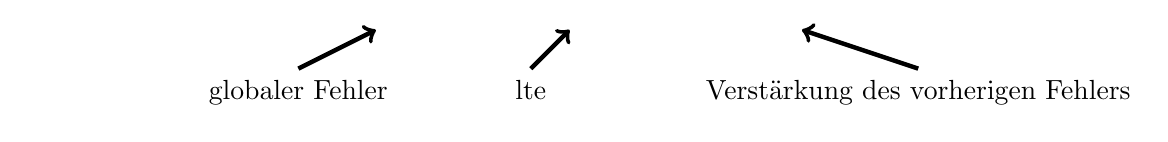
\begin{tikzpicture}
	\centering
	\node[anchor=south west,inner sep=0] (Bild) at (0,0){};
	\begin{scope}[x=(Bild.south east),y=(Bild.north west)]
		\draw [ultra thick] [->] (70,0) -- (90,10) node [pos=0,below] {globaler Fehler};
		\draw [ultra thick] [->] (130,0) -- (140,10) node [pos=0,below] {lte};
		\draw [ultra thick] [->] (230,0) -- (200,10) node [pos=0,below] {Verst\"arkung des vorherigen Fehlers};
	\end{scope}
\end{tikzpicture}

\subsubsection{Konvergenz}
Eine Finite-Differenzen Methode ist konvergent, wenn f\"ur jede Konstante $n\delt = T = const.$ gilt:
\begin{equation*}
	\|E^n\| = \|\overline{u}^n - u^n\| \xlongrightarrow[\text{$\Delta$} t \text{, $\Delta$}x -> 0]{n\text{$\Delta$}t = T = const.} 0
\end{equation*}
Allgemein ist die Simulation nur zuverl\"assig, wenn diese Konvergent ist. Das l\"asst sich wie folgt beweisen:\\
Lax-Richtmayer \"Aquivalenz Theorem:\\
Konstistenz + Stabilit\"at = Konvergenz
\begin{equation*}
	\|E^{n+1}\| \leq \|\overline{u}^{n+1}_i - L\cdot \overline{u}^n\| + \|L\cdot \overline{u}^n + L\cdot u^n\| \leq \delt \sum O(\dex^p\delt^q) + \|\|\overline{u}^{n+1}_i - u^n\| \leq ... \leq (n\delt) \sum O(\dex^p\delt^q) + \|E^0\|
\end{equation*}
\par
\vspace{-2em}
\begin{tikzpicture}
	\centering
	\node[anchor=south west,inner sep=0] (Bild) at (0,0){};
	\begin{scope}[x=(Bild.south east),y=(Bild.north west)]
		\draw [ultra thick] [->] (290,0) -- (310,10) node [pos=0,below] {Konsistenz-(Kovergenz-)Ordnung};
	\end{scope}
\end{tikzpicture}

